
\section{Calibration}


The model is calibrated to a quarterly frequency. There are three goals to the parameterization of households. The first is to match the earnings loss following job displacement documented in \cite{DavisVonWachter2011}. The second is to simultaneously match a large aggregate MPC consistent with micro estimates while also matching aggregate liquid wealth in the 2007 Survey of Consumer and Finances. I choose the 2007 survey as I aim to match The Great Recession in section 7. The third is to match labor market transition probabilities of permanent layoffs, temporary layoffs, other types of unemployment from estimated in \cite{Gertler2022}. The parameterization of households is broken into two steps. I first calibrate all parameters excluding the discount factors. I then estimate three uniformly distributed discount factors to match the aggregate liquid wealth from the 2007 SCF and a quarterly MPC of 0.21 as in \cite{kekre2023}. The remaining parameters are calibrated to standard values in the New Keynesian and search and matching literatures. 
 

\hypertarget{Households}{}
\subsection{Households }


\textbf{Labor transition probabilities}    The job separation rate $\omega$ is set to 0.1 in line with JOLTS. I set the job finding probability of households separated in the current period, $\eta_{r,t}$,  to 0.675 to target an employment to unemployment (EU) transition probability of 4.1\%, the estimate of the monthly EU probability in \cite{Gertler2022} (henceforth GHT) aggregated to a quarterly frequency. The probabilities of becoming a permanent layoff $\gamma_{P}$, a temporary layoff $\gamma_{P}$, and a quitter/other $\gamma_{O}$, are calibrated to match the EU probabilities of entering each unemployment state estimated in GHT and \cite{GHT2023}\footnote{\cite{Gertler2022} estimate the E to U probability of entering a permanent separation and a temporary layoff while \cite{GHT2023} estimate the E to U probability of entering as a layoff or as a quitter/other. Both papers use the CPS from 1976 to 2019, and the same methodology, to estimate the transition probability between both different unemployment states. In addition, the estimation of both papers yield the same mean unemployment rate, the same E to E probability, and the same E to inactive probability. The probability of E to U in both papers are similar as well.  I use estimates of both papers to deduce the E to U probability of permanent layoffs, temporary layoffs, and quits/others.}. The job finding probabilities of each unemployment state $\eta_{t}(X)$ is calibrated the estimated monthly job finding probabilities in GHT, aggregated to a quarterly frequency. I let the job finding probability of permanent layoffs and quits/others to equal the estimate of the job finding probability of permanent separators in GHT as they do not distinguish between permanent layoffs and quits/others. The probability of transitioning from temporary layoff to permanent layoff, $P_{TLPL}$,  is set to 0.47 which follows from the estimate in (GHT). The resulting steady state unemployment rate is $6.2 \%$, equal to the mean unemployment rate estimated from the Current Population Survey in GHT.  I calibrate $\zeta_{P}$, $\zeta_{T}$, and $\zeta_{O}$ such that permanent layoffs, temporary layoffs, and quits/others, account for $63\%$, $20\%$, and $17\%$, respectively, of an increase in the unemployment rate. GHT estimate the distribution of the increase in the unemployment rate from trough to peak across permanent separations and temporary layoffs for during the Great Recession. Their estimates indicate that the average increase in unemployment that is attributed to temporary layoffs is $17\%$. For increases in the unemployment rate attributed to quits/others and permanent layoffs, I use the decomposition of unemployment by reason constructed by \cite{Fujita2017} using data from the BLS. Using the \cite{Fujita2017} series, I calculate that during the Great Recession, $20\%$ of the increase in the unemployment rate from trough to peak are attributed to reentrants and use this as my target for the quits/others group as my model does not include inactive/out of the labor force as a state. I assign the remaining proportion of the increase in the unemployment rate is attribute to the permanent layoffs unemployment type. \\


\textbf{Human Capital Dynamics}  I use an equally spaced grid with the maximum value of human capital, $\bar{h}$, to 1.8 and the minimum value, $\underline{h}$, to 0.2 as in \cite{Birinci2021}. I set the number of human capital grid points to 20 and assume $\Delta_{L} = 0.1$ so that when an employed household accumulates capital it increases by one grid point. The probability of human capital erosion during unemployment $\pi_{U}$ is set to 0.75 as in \cite{Birinci2021}. I then estimate the magnitude of human capital erosion, $\Delta_{U}$ and the probability of human capital accumulation during employment, $\pi_{L}$ to minimize the distance between the earnings loss following job loss in the model and the earnings loss following job loss during recessions estimated by \cite{DavisVonWachter2011}. I target the estimate of earnings loss following job loss in recessions as I will later simulate all past recessions since the 1980s. The resulting estimation yields  $\Delta_{U} = 0.3$ and $\pi_{L}=0.085$. \\

\textbf{Income process}    The calibration of permanent and transitory income shock distributions follow \cite{carroll2017distribution} with the standard deviation of permanent shocks set to $0.06$ and the standard deviation of transitory shocks set to $0.2$. The real wage is normalized to 1.0 and the real wage rigidity parameter $\phi_{w} = 0.837$ as in \cite{Gornemann2021}. The unemployment insurance replacement rate is set to 50\%. The income parameters that dictate the amount of non-UI income and government transfers, $\omega_{1}$, $\omega_{2}$, and $T^{s}$, are calibrated to match microeconomic moments on household income throughout unemployment documented in \cite{kekre2023}. In particular, these parameters are calibrated such that total income of unemployed households who receive UI is $76\%$ of pre job loss income, total of income of unemployed households who do not receive UI is $55\%$ of pre job loss income, and government transfers capture $13\%$ of pre job loss income of households who have been unemployed for longer than two quarters. \\

\textbf{Discount Factor Estimation}  Following \cite{carroll2017distribution}, households are ex-ante heterogenous in their discount factors. I let three discount factors, $(\bar{\beta} - \nabla, \bar{\beta} , \bar{\beta} + \nabla)$ , be uniformly distributed across the population. I estimate the mean discount factor, $\bar{\beta}$, to target the aggregate liquid wealth to aggregate quarterly permanent income ratio in the 2007 Survey of Consumer Finances and the spread, $\nabla$, to target an aggregate quarterly MPC of 0.21 as in \cite{kekre2023}. Following \cite{Kaplan_Brookings}, I define liquid wealth as checking, saving, money market and call accounts as well as directly held mutual funds, stocks, corporate bonds, government bonds less credit card balances. I restrict my sample of liquid wealth to households with nonnegative liquid wealth as the model does not feature borrowing.  I also remove all households with zero permanent income. Table 1 presents the estimated discount factors. \footnote{This is consistent with the work of Allcott et al. (2021) and Skiba and Tobacman (2009), who estimate discount factors  of 21\% at a 2 week frequency and discount factors between 0.74 to 0.83 at a 8 week frequency, respectively. Although both papers assume hyperbolic discounting, the point is that a very low discount factor is needed to match the proportion of the population who are willing to take out payday loans at very high interest rate. }

\begin{table}[H]
\begin{center}\renewcommand{\arraystretch}{2.0}
\caption{Discount factor estimates}\label{table:DiscFacEstimation}
\begin{tabular}{ccccccc}
\hline
      \multicolumn{7}{c}{ Discount Factors }    \\ \hline
   .937   & .964 &   .991 \\   
 \hline
\end{tabular}
\end{center}
\end{table}

\textbf{Remaining Parameters} I let $U(c) = \frac{ c ^ { 1-\rho } } {1-\rho}$ and I set the CRRA parameter, $\rho$, to 2 and the probability of death to .00625 match a 40 year work life. The real rate is $3\%$ annualized.

\subsection{Rest of the Economy }

The quarterly vacancy filling rate is 0.71 as in \cite{Wouter2000}. The matching elasticity is 0.65 following \cite{ravn2017job} and the vacancy cost is set to 7\% of the real wage as in \cite{Christiano2016}\footnote{The range of plausible values lie between $4\%$ and $14\%$ as documented in \cite{SilvaToledo}}. The elasticity of substitution is set to 6. The price adjustment cost parameter is set to 96.9 as in \cite{ravn2017job}. The tax rate is set to 0.3 and government spending is set to clear the government budget constraint.  I follow \cite{AuclertMicroJumpsMacroHumps} in calibrating the fiscal adjustment parameter  as well as the decay rate of government coupons by setting $\phi_{b} = 0.1$ and $\delta = 0.95$ to match a maturity of 5 years\footnote{The duration of bonds in the model is $\frac{(1+r)^4}{(1+r)^4 - \delta}$ }.


\begin{center}
\renewcommand{\arraystretch}{1.7}
\begin{table}[H]
\centering
\caption{Household Calibration}\label{table:Calibration}
\makebox[\textwidth]{\begin{tabular}{c c c l}
Description & Parameter & Value & Source/Target \\ 
\hline
CRRA & $\rho$ & 2 & Standard \\
Real Interest Rate & $r$ & $1.03^{\frac{1}{4}} - 1$ & 3\% annualized real rate \\
Probability of Death & $D$ & 0.00625 & 40 Year Work Life \\
\begin{small}$\frac{\text{Liquid Wealth}}{\text{Quarterly Permanent Income}}$ \end{small} & $\frac{A}{\Phi}$ & 4.4 & 2007 Survey of Consumer Finances \\
\hline 
Prob. of human capital accumulation & $\pi_{L}$ & 0.085 & See text \\ 
Prob. of human capital erosion & $\pi_{U}$ & 0.75 & \cite{Birinci2021} \\  
Human capital accumulation step & $\Delta_{L}$ & 0.1 & Normalized \\ 
Human capital erosion step & $\Delta_{U}$ & 0.3 & See text \\  
\hline
Tax Rate & $\tau$ & 0.3 & \cite{kaplan2018monetary} \\
Real Wage & $w$ & 1.0 & Normalized \\
UI replacement rate & $b$ & 0.5 & 50$\%$ replacement rate \\
Non UI income parameter 1 & $\omega_{1}$ & 0.182 & \begin{footnotesize}$ \frac {\text{HH income w. UI} }{ \text{pre job loss income} } = 0.76$ \end{footnotesize} \\
Non UI income parameter 2 & $\omega_{2}$ & 0.294 & \begin{footnotesize} $\frac{\text{HH income w.o. UI}}{\text{pre job loss income}} = 0.55$ \end{footnotesize} \\
Gov. transfers & $T_{s}$ & 0.091 & \begin{footnotesize} $\frac{\text{SNAPS and Soc. Security Inc}}{\text{Pre Job Loss Income}} = 0.13$ \end{footnotesize} \\
Std Dev of Log Permanent Shock & $\sigma_{\psi}$ & 0.06 & \cite{carroll2017distribution} \\%\cite{carroll2017distribution} \\
Std Dev of Log Transitory Shock & $\sigma_{\theta}$ & 0.2 & \cite{carroll2017distribution}  \\ \hline %\cite{carroll2017distribution} \\  \hline
\end{tabular}}
\end{table}
\end{center}

\begin{center}
\renewcommand{\arraystretch}{1.7}
\begin{table}[H]
\centering
\caption{Labor Transition Calibration}\label{table:Calibration}
\makebox[\textwidth]{\begin{tabular}{c c c l}
Description & Parameter & Value & Source/Target \\ 
\hline
Job Separation Prob. & $\omega$ & 0.1 & JOLTS \\
Job Finding Prob. of recently separated & $\eta_{r,t}$ & 0.59 & EU probability of $4.1\%$ \\ 
Job Finding Prob. of perm. layoff & $\eta_{t}(P)$ & 0.51 & \cite{Gertler2022} \\ 
Job Finding Prob. of temp. layoff & $\eta_{t}(T)$ & 0.82 & \cite{Gertler2022} \\ 
Job Finding Prob. of quit/other & $\eta_{t}(O)$ & 0.51 & \cite{Gertler2022} \\ \hline
Prob. of perm. layoff in steady state & $\lambda^{P}_{ss}$ & 0.35 & $35\%$ of EU from perm. layoffs \\ 
Prob. of temp. layoff in steady state & $\lambda^{T}_{ss}$ & 0.31 & $31\%$ of EU from temp. layoffs \\ 
Prob. of quit/other in steady state & $\lambda^{O}_{ss}$ & 0.33 & $33\%$ of EU prob. quit/other layoffs \\ \hline
Perm. layoff deviation param. & $\zeta^{P}$ & 10.3 & $63\%$ of $\Delta$ Urate from perm layoffs \\ 
Temp. layoff deviation param. & $\zeta^{T}$ & -4.4 & $17\%$ of $\Delta$ Urate from temp layoffs \\ 
Quits/other layoff deviation param. & $\zeta^{O}$ & -5.9 & $20\%$ of $\Delta$ Urate from quits/other \\ \hline

\end{tabular}}
\end{table}
\end{center}

\begin{center}
\begin{table}[H]
\renewcommand{\arraystretch}{1.6}
\caption{Rest of Economy Calibration}\label{table:Calibration}
\makebox[\textwidth]{\begin{tabular}{c c c l}
Description & Parameter & Value & Source/Target \\ \hline
Elasticity of Substitution & $\epsilon_{p}$ & 6 & Standard \\
Price Adjustment Costs & $\varphi$ & 96.9 & \cite{ravn2017job} \\
Vacancy Filling Rate & $\phi$ & 0.71 & \cite{Wouter2000} \\
Matching Elasticity & $\alpha$ & 0.65 & \cite{ravn2017job} \\
Real Wage Rigidity parameter & $\phi_{w}$ & 0.837 & \cite{Gornemann2021} \\
Vacancy Cost & $\kappa$ & 0.056 & $\frac{\kappa}{w\phi} = 0.07$ \\
Government Spending & $G$ & 0.38 & Gov. budget constraint \\
Decay rate of Government Coupons & $\delta$ & 0.95 & 5 Year Maturity of Debt \\
Taylor Rule Inflation Coefficient & $\phi_{\pi}$ & 1.5 & Standard \\
Response of Tax Rate to Debt & $\phi_{b}$ & 0.1 & \cite{AuclertMicroJumpsMacroHumps} \\ \hline
\end{tabular}}
\end{table}
\end{center}



\section{Model Validation: Persistent Earnings Loss Following Unemployment}

In this section, I verify the model generates persistent earnings loss following job displacement that matches the estimates in \cite{DavisVonWachter2011}. 

To evaluate the path of earnings loss following job displacement, I run a regression similar to \cite{DavisVonWachter2011} with the same sample restrictions on model simulated data. Since the model is calibrated to a quarterly frequency, I aggregate the simulated data to a yearly frequency. For a given year $b$, the sample of displaced workers constitutes households who enter unemployment in year $b, b+1$, or $b+2$.  Households who do not enter employment during year $b, b+1$, or $b+2$ constitute the sample of non displaced workers. I restrict the the sample to households who have been continuously employed for 6 years prior to year $b$\footnote{When aggregating to annual frequency, a worker who was unemployed  for at least one quarter is denoted as displaced for that year. and is therefore not considered as employed for that year.}. With these sample restrictions, I run the following regression on simulated data.


$$
log(z_{iy}^{b}) = c^{b} + \Sigma_{k\geq -6}^{20}  \delta_{k}^{b} D_{iy}^{k} + \epsilon_{iy}^{b}
$$  

where $z_{iy}$ is labor income, $D_{iy}^{k}$ is a indicator denoting a household that was displaced $k$ years ago, and $c$ is a constant in the regression. The regression features no fixed effects as human capital is exogenous with respect to becoming unemployed.  $\delta_{k}$ for $k = 1, 2, ....,20$ are the key estimates that capture the earnings of an individual who was displaced $k$ years ago compared to an individual who was not displaced $k$ years ago. 
\begin{figure}[H]
    \centering
     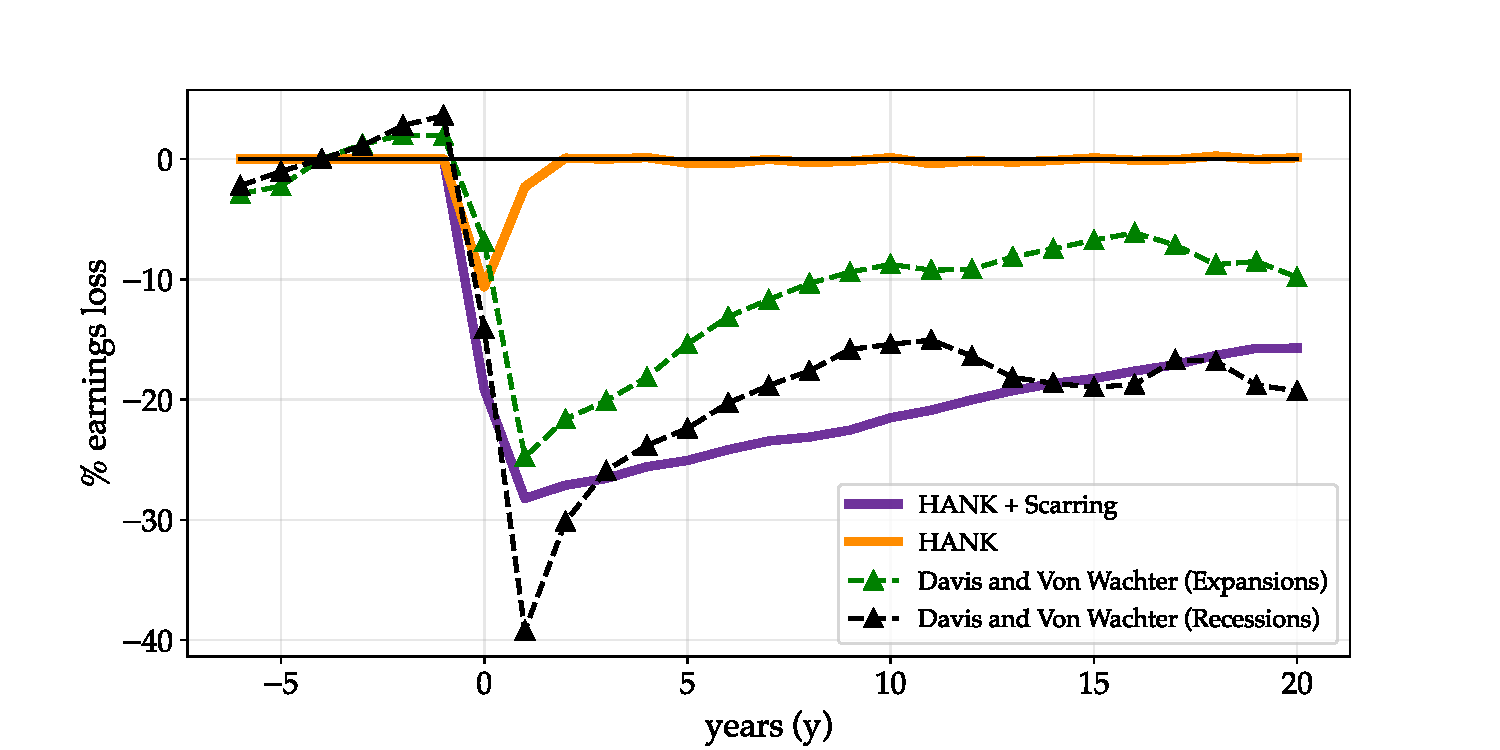
\includegraphics[scale=.65]{text/chapter1/Figures/Scarring_match}
      \caption{Earnings loss following job loss in $y=0$: Model vs Data}
 \label{Scar_match_PE}
\end{figure}
Figure \ref{Scar_match_PE}  illustrates the path of earnings loss following displacement for the baseline model with scarring (HANK + Scarring) and the model without scarring (HANK). Scarring is eliminated by assuming the probability of accumulation or erosion in human capital is eliminated. The baseline model produces a severely persistent earnings loss that is missing in the model without human capital dynamics. As in the data, these losses remain after 20 years. 

